\chapter{Results}
\label{section:7_Results}

This chapter presents a more accurate description of the results obtained in~\cref{section:Parameters_to_SXR} as they represents an actual implementation of most of the ML methods presented so far.
The structure that has been applied is the same reported in~\Figure{\ref{fig:SXR_from_param}} where a Variadic Autoencoder has been joined with a standard inference network to map the the magnetic configuration into the SXR latent space reconstruction, and than this latent configuration back to the SXR representation.

\section{Relevance layer}

The structure of the networks that have been used to construct these results starts from a \VAE{6} (autoencoder with a latent dimension of 6) and a inference network converting a generic feature from other sensors into that latent set.
These are the same structures that have been applied to obtain the previous results, but a further layer has been added to networks. Although based on a very simple idea, this layer is not coming from a standard ML methodology, so we decided to discuss it here. 

The idea comes from the observation that the at a certain point we needed to decide which plasma parameters had to be fed in the inference network to reconstruct the latent state. Obviously the selected parameters started from a guess of a sufficient information on the physical model that links the magnetic configuration to the temperature profile, even if in this case a complete mapping is not available.
% SPIEGARE QUI PERCHE'
In the limit of a reasonable number of inputs we decided to be create a rich set starting from some standard parameters, like the plasma current ($I_p$), toroidal loop potential ($V_t$), the reversal ($F$) and the ration of the dominant mode over secondaries ($NS$). Beside these a complete description, in argument and phase, of 15 modes from m=1 perturbation should provide the needed plasma shape to the network making it able to identify the position and the amplitude of the QSH.

However to define which are the most relevant parameters that play a role in the description of the plasma temperature we decided to turn the problem upside down. The idea indeed it to make the network itself yielding this from the training. Thus this layer is a simple dense perceptron where the linear pass through activation and an \textbf{identity matrix} for the weights. The point is that this is the former layer of the network, directly attached to the input features, and the weights are trainable. The layer definition needs also to constrain the initialization to set the identity and to fix all the other link to be kept to zero. 

Then during training the backpropagation tends to create a selection automatically by suppressing the inputs that are not contributing to the reduction of the loss, i.e. that does not correlate with the temperature profile.
So along the training epochs the loss, and possibly all the further regularization added, gradually silence that signals. This provides, not only a further layer that masks the non relevant inputs, bus once the weights are eventually exposed a short of "relevance" meter that can tell what inputs the target is more sensible at.
%
\begin{figure}
    \centering
    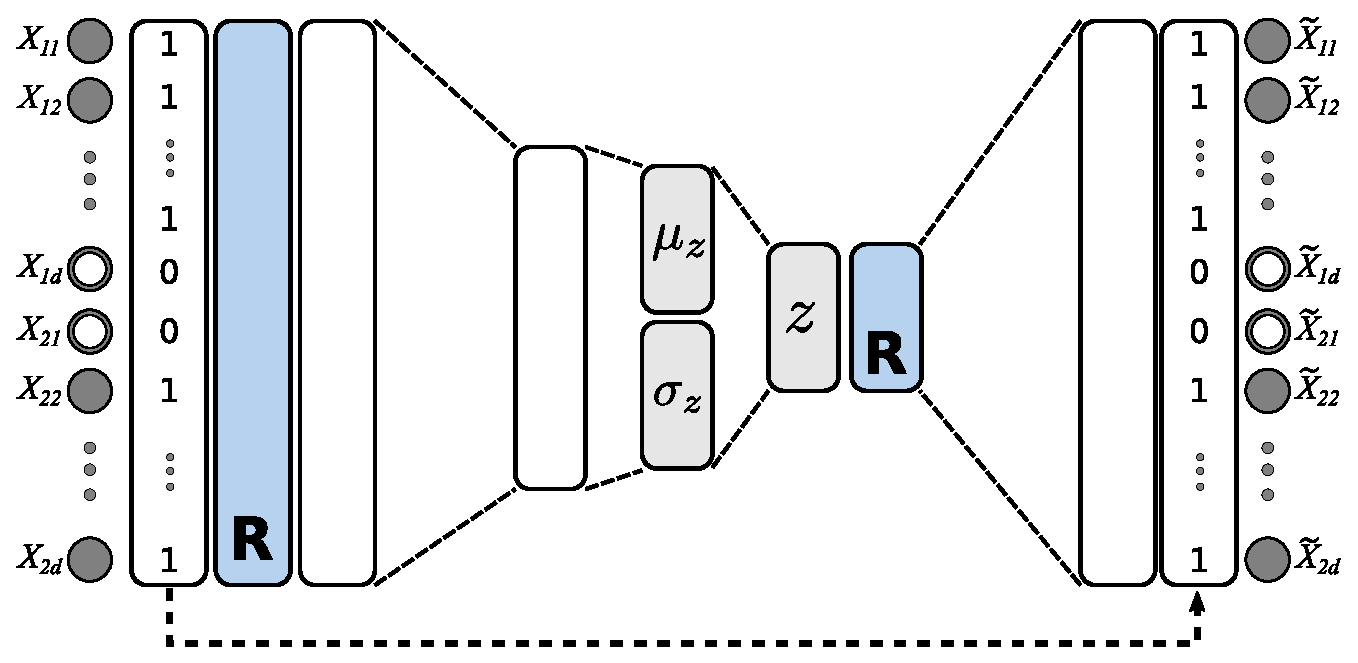
\includegraphics[height=6cm]{img/STEP12_7/VAE_RELEVANCE.eps}
    \caption{Relevance layer}
    \label{fig:relevance}
\end{figure}
%
The implemented idea is shown schematically in \Figure{\ref{fig:relevance}}, where the basic schema of a VAE with missing input is presented. The new relevance layers, shown with the (R) mark on the picture, can be placed after the input feature layer (just after the NaN-Mask layer) and/or at the latent space layer (the first layer of the decoder).
Although the picture shows the case of an Autoencoder, the same layer can be applied to a simple inference too.
In the case of the Autoencoder the first relevance layer will provide the amount of mutual information that each particular input has with the others, while the second will give a hint on how much the encoder is providing a disentangled representation because the redundant dimension are kept out from the generative process.
On the other hand the simple application on a standard regression network such the one that we used to pass from magnetics to the temperature profiles provides the actual significance of each input parameter to the task of building the guess.

A sparsity promotion regularizer, such as the dropout, beside the effects on the network generalization, shown to improve the relevance too.
%
\begin{figure}
    \centering
    \subfigure{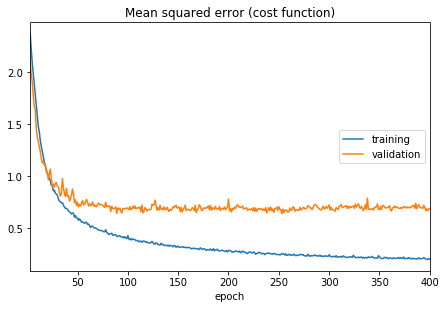
\includegraphics[height=3.3cm]{img/STEP12_7/STEP12_7_pBr2SXR_rm-rs_absarg_training_mse.png} \label{step_12_7_training}}
    \subfigure{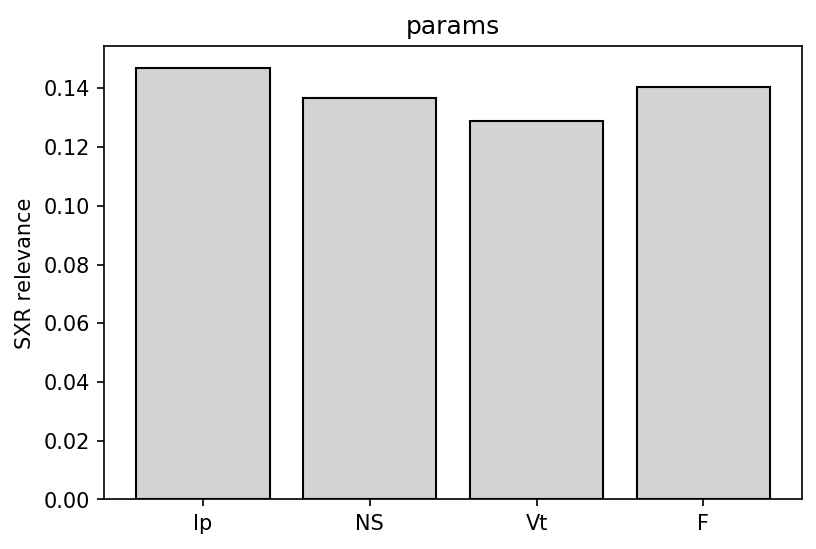
\includegraphics[height=3.3cm]{img/STEP12_7/STEP12_7_params.png} \label{fig:step_12_7_p}}
    \subfigure{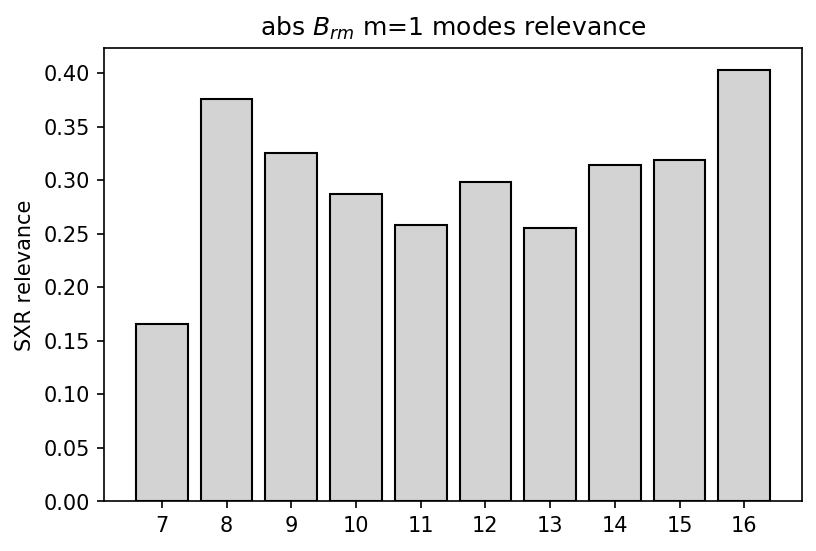
\includegraphics[height=3.3cm]{img/STEP12_7/STEP12_7_abs_Br_rm.png} \label{fig:step_12_7_abs_Brm}}
    \subfigure{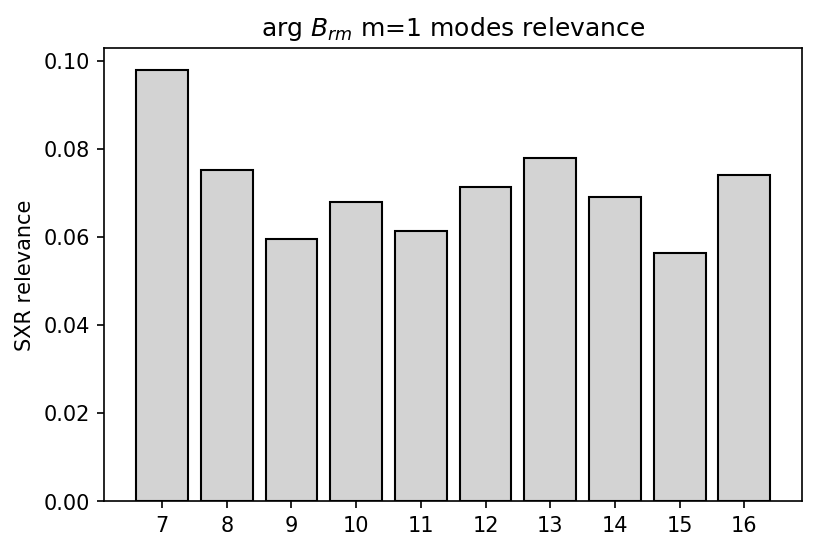
\includegraphics[height=3.3cm]{img/STEP12_7/STEP12_7_arg_Br_rm.png} \label{fig:step_12_7_arg_Brm}}
    \subfigure{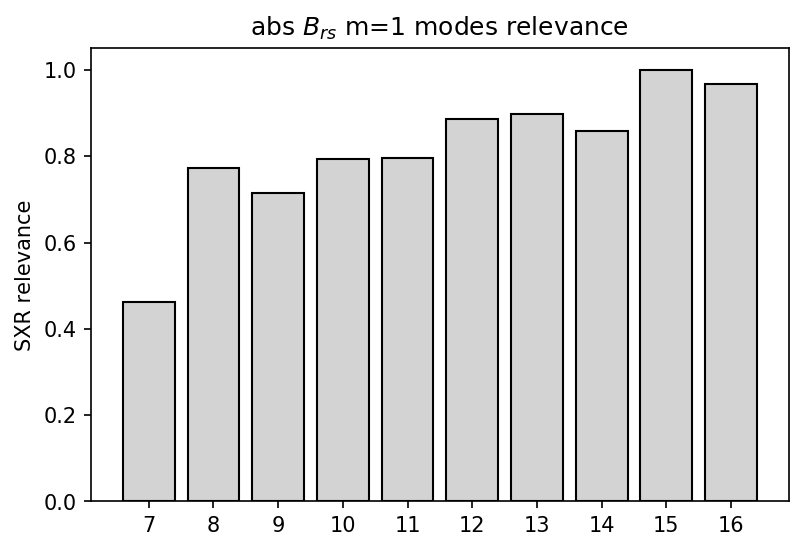
\includegraphics[height=3.3cm]{img/STEP12_7/STEP12_7_abs_Br_rs.png} \label{fig:step_12_7_abs_Brs}}
    \subfigure{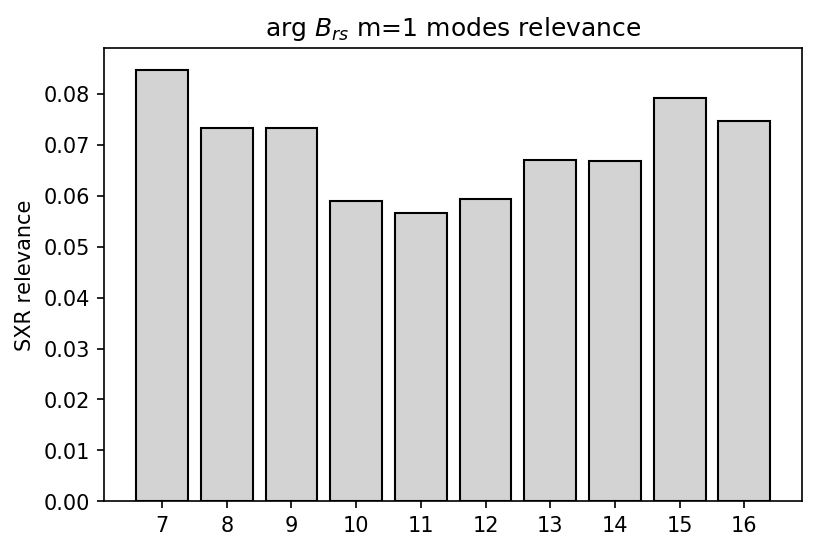
\includegraphics[height=3.3cm]{img/STEP12_7/STEP12_7_arg_Br_rs.png} \label{fig:step_12_7_arg_Brs}}
    \caption{ Training 500 epochs - STEP 12.7 mse, slightly overfitted but validation not diverging }
    \label{fig:step_12_7_relevance}
\end{figure}
%
In \Figure{\ref{fig:step_12_7_relevance}} the training process for the parameters inference is presented, together with the obtained relevance values for all the inputs.
These results are not yet conclusive, although the expected dependence on the m=1 n=-7 phase is at least confirmed.
To obtain a more informative result a better use of regularization will be necessary possibly also characterizing the all values from a sequence of repeated training on the network.

\section{EM to SXR mapping results}

The implementation of the network structure follow the example already discussed in~\cref{section:Parameters_to_SXR}.
For the initial latent representation of the SXR3 temperature signal a \bVAE{6} has been used with only dense layers. We started by a balanced 15 points dataset, composed of the impact position (x-axis) and temperature value (y-axis) of the measured $T_e$ along 45K acquisitions in random order. The input has been unfolded on a single feature array of 30 values similarly to what discussed in \cref{section:SXR_dataset}. The \bVAE{6} is composed by the following simple topology. For the encoder: NaN-Mask layer, Relevance layer with dropout, 4 ReLU dense layers with normalization and dropout, and 6 linear units for gaussian stochastic latent variables. For the decoder: 4 ReLU dense layers with the final one with linear activation output. The four layers of encoder and decoder have been constructed with the automatic shaping geometry of: \texttt{2 x [20,20,10,10]}. This yields symmetric structures with: $(1.2, 1.2, 0.6, 0.6) \times 10^3$ units and $(0.6, 0.6, 1.2, 1.2) \times 10^3$ for the two networks respectively.
The dropout rate for training has been set to $10^{-1}$ while $\beta=10^{-3}$ has been set for the KL term of VAE.

Once trained the \VAE{6} latent space has been used as a label for training a further inference network where the features were in order: the plasma current ($I_p$), the ratio of the dominant mode over secondaries ($NS$), the toroidal loop potential ($V_t$), the reversal factor ($F$), and the magnitude and phase of $B_r$ and $B_\varphi$ for $m=0, n=[-7 \tilde -15]$ modes extrapolated to the sensors position and cleaned of the toroidal side-bands with the procedure described in~\cite{Zanca_2004}.
The resulting network is composed by 44 inputs and 6 outputs. We chose the same geometry of the VAE that resulted in 4 ReLU dense layers with $(1.76, 1.76, 0.88, 0.88) \times 10^3$ units. 

The dataset has been divided in a 3K samples for validation and the remaining for the training. The training has been performed with 500 epochs with 446 minibatches of 100 samples each. The training has been performed on a standard workstation Intel(R) Core(TM) i7-4770 3.40GHz taking approximately 220ms per step and 98s per epoch. The network resulted to be slightly overfitted, but the validation error did not diverge though. This effect, visible in \Figure{\ref{fig:fig:step_12_7_p}} has been observed on all the tests executed so far so we decided to continue the training over the early stopping position until the plateau of the validation.

Some resulting reconstruction are reported in \Figure{\ref{fig:Step_12_val}} where 6 examples have been reported taking 6 samples from the validation dataset. The pictures are organized in rows: the first plot is a direct comparison of the real temperature and the reconstructions, the second is a 2D countour of the magnetic flux reconstruction made with SHEq code~\cite{Martines_2011}, the last is instead a histogram of some plasma parameters averaged over the corresponding pulse and time window that pertains to the acquired temperature profile.
%
\begin{figure}
\centering

a.\subfigure{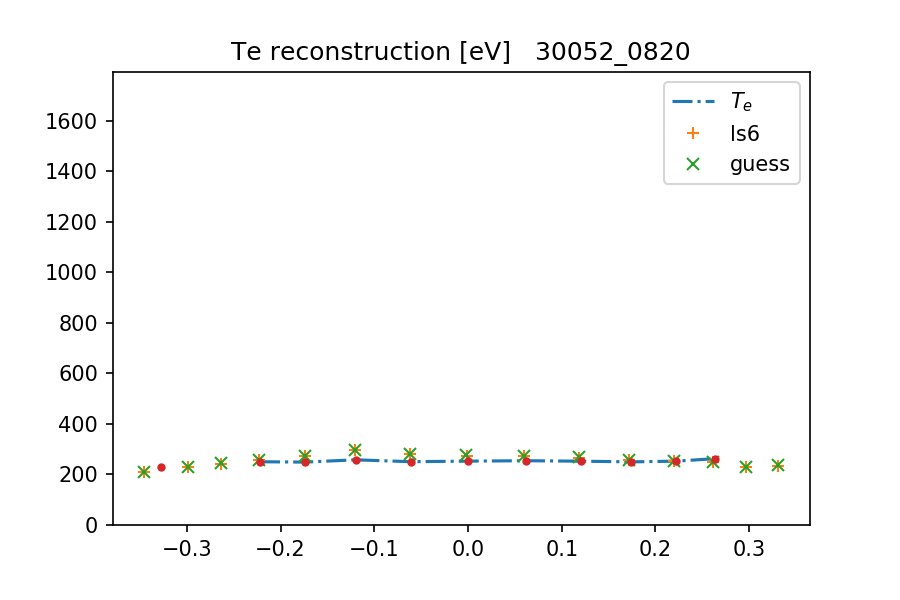
\includegraphics[height=4cm,trim={0.5cm 0cm 0.5cm 0.5cm},clip]{img/STEP12_7c/Te_rec_16.png}   }%    
\subfigure{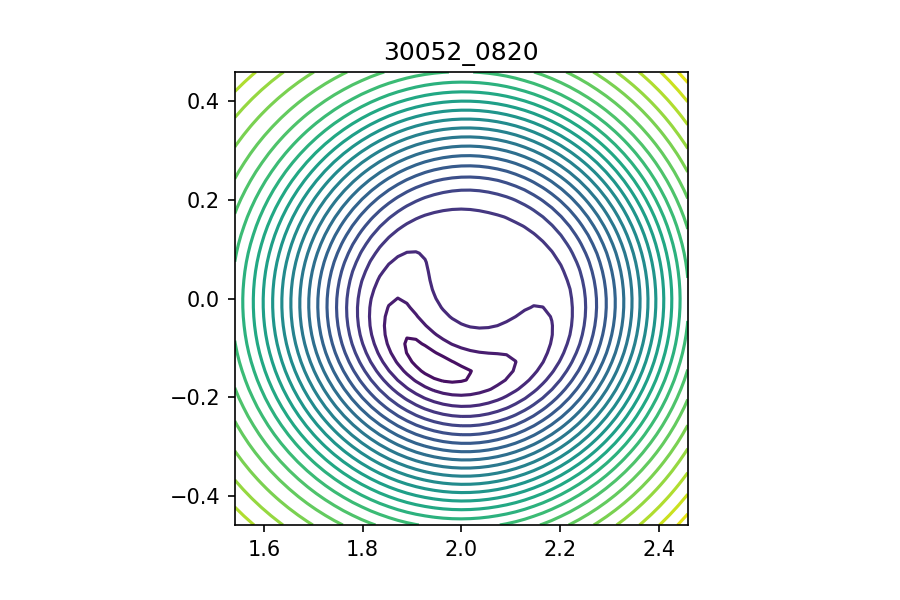
\includegraphics[height=4cm,trim={3cm   0   3.5cm 0    },clip]{img/STEP12_7c/Contour_16.png}  }%   
\subfigure{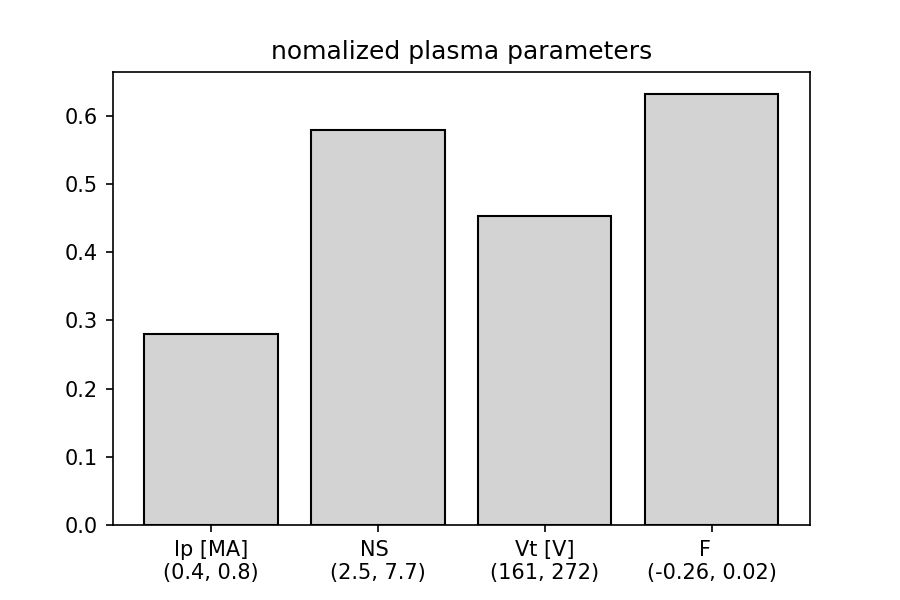
\includegraphics[height=4cm,trim={0.5cm 0cm 0.5cm 0cm  },clip]{img/STEP12_7c/Params_16.png}   }\\%
b.\subfigure{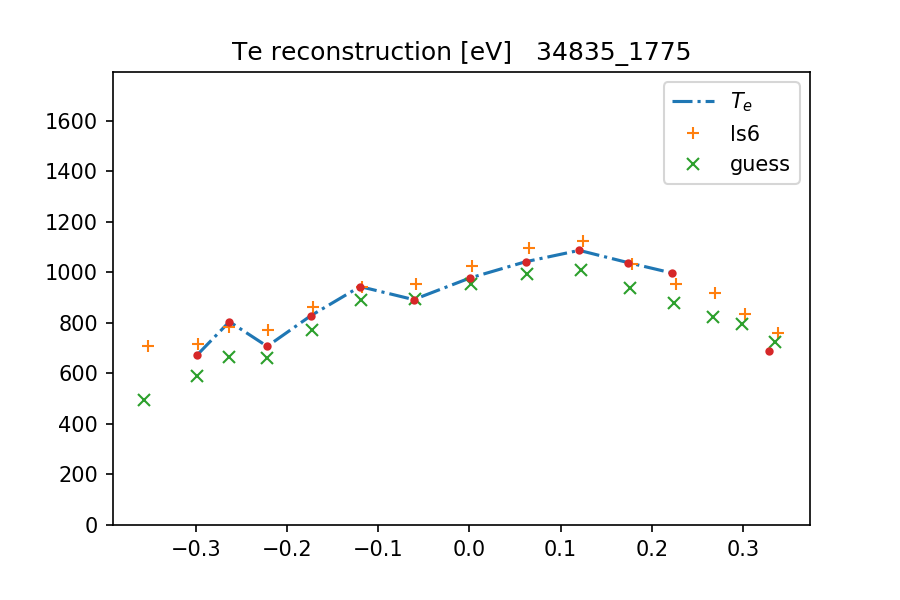
\includegraphics[height=4cm,trim={0.5cm 0cm 0.5cm 0.5cm},clip]{img/STEP12_7c/Te_rec_143.png}  }%   
\subfigure{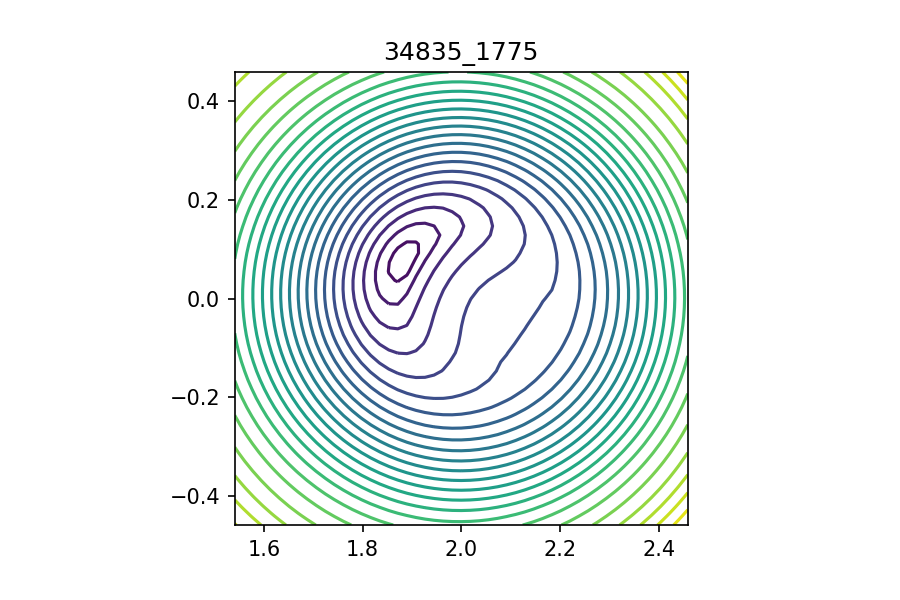
\includegraphics[height=4cm,trim={3cm   0   3.5cm 0    },clip]{img/STEP12_7c/Contour_143.png} }%  
\subfigure{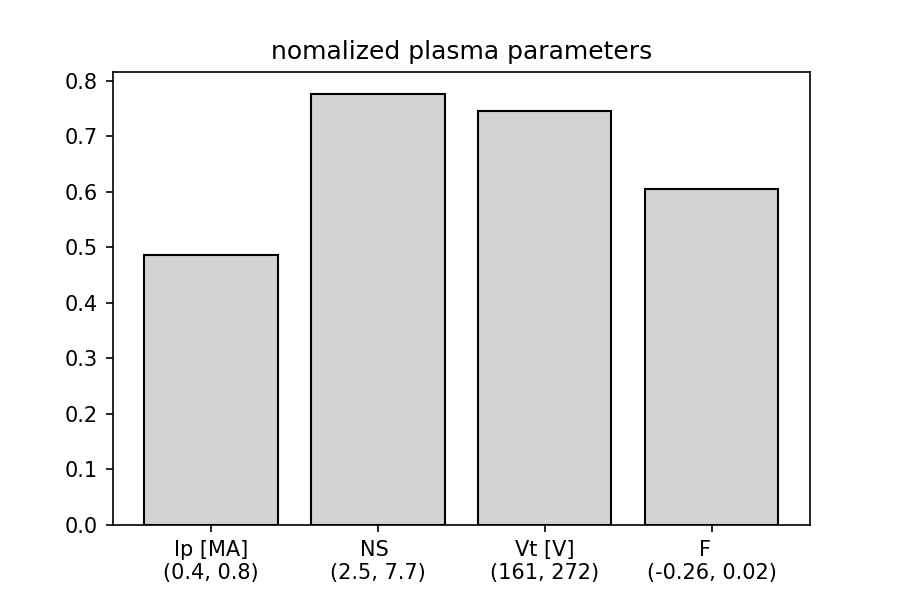
\includegraphics[height=4cm,trim={0.5cm 0cm 0.5cm 0cm  },clip]{img/STEP12_7c/Params_143.png}  }\\%
c.\subfigure{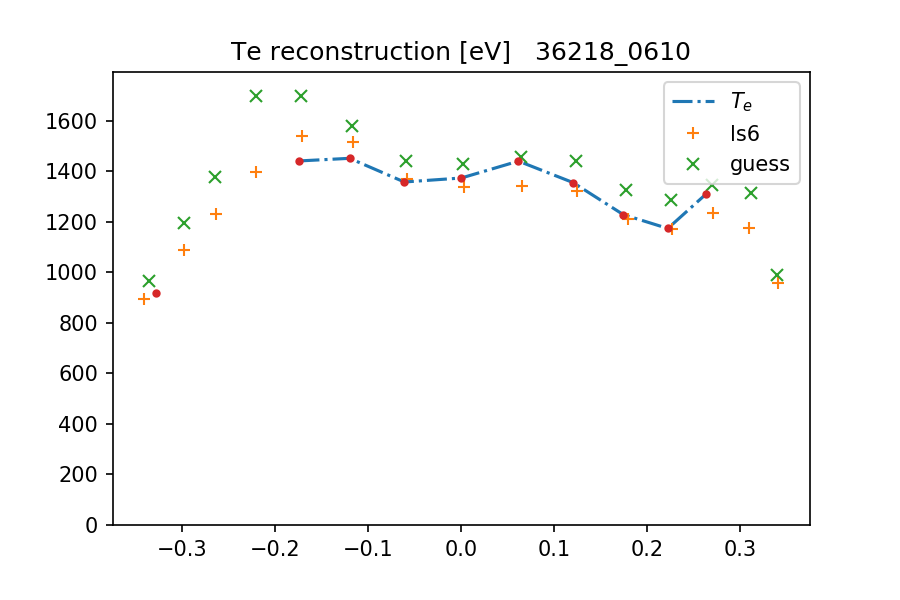
\includegraphics[height=4cm,trim={0.5cm 0cm 0.5cm 0.5cm},clip]{img/STEP12_7c/Te_rec_201.png}  }%   
\subfigure{\includegraphics[height=4cm,trim={3cm   0   3.5cm 0    },clip]{img/STEP12_7c/Contour_201.png} }%  
\subfigure{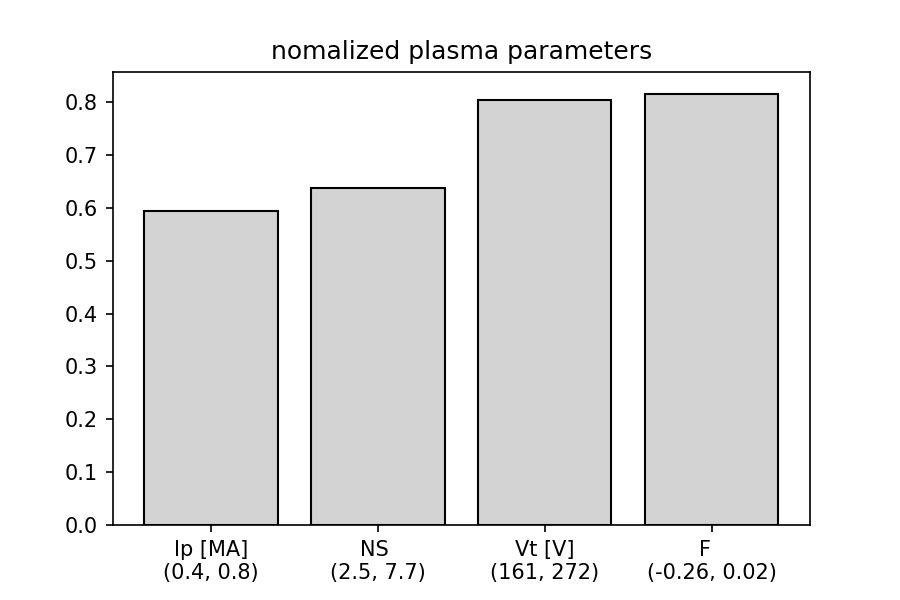
\includegraphics[height=4cm,trim={0.5cm 0cm 0.5cm 0cm  },clip]{img/STEP12_7c/Params_201.png}  }\\%
d.\subfigure{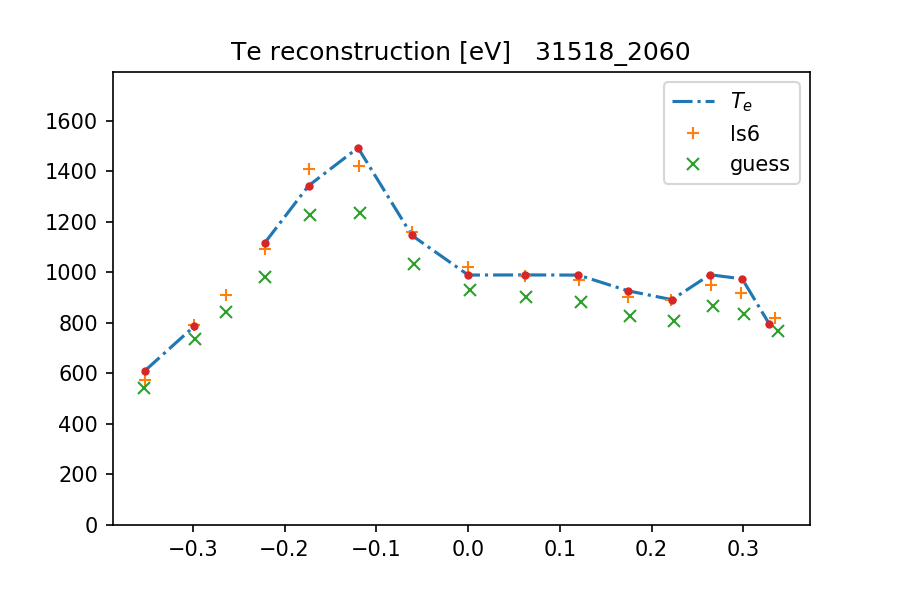
\includegraphics[height=4cm,trim={0.5cm 0cm 0.5cm 0.5cm},clip]{img/STEP12_7c/Te_rec_160.png}  }%   
\subfigure{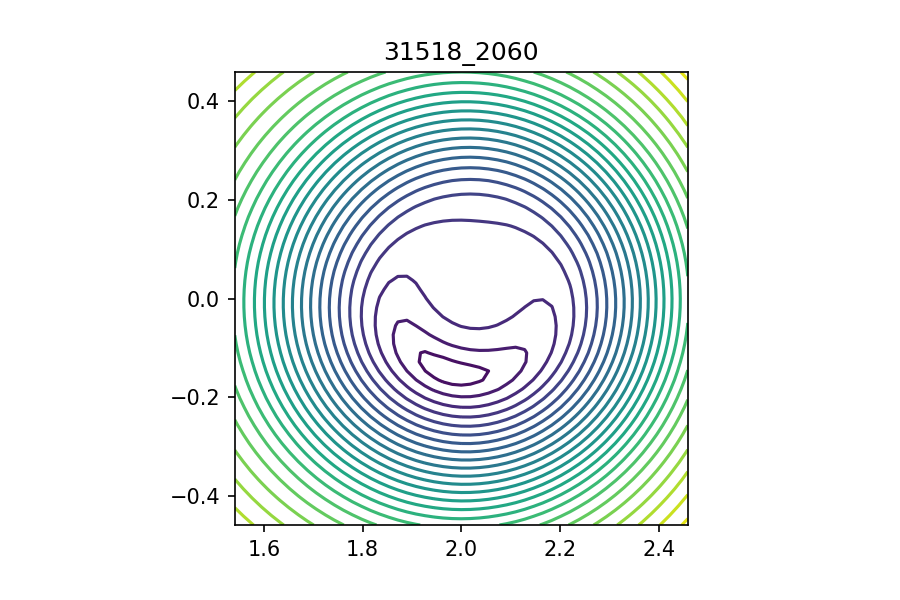
\includegraphics[height=4cm,trim={3cm   0   3.5cm 0    },clip]{img/STEP12_7c/Contour_160.png} }%  
\subfigure{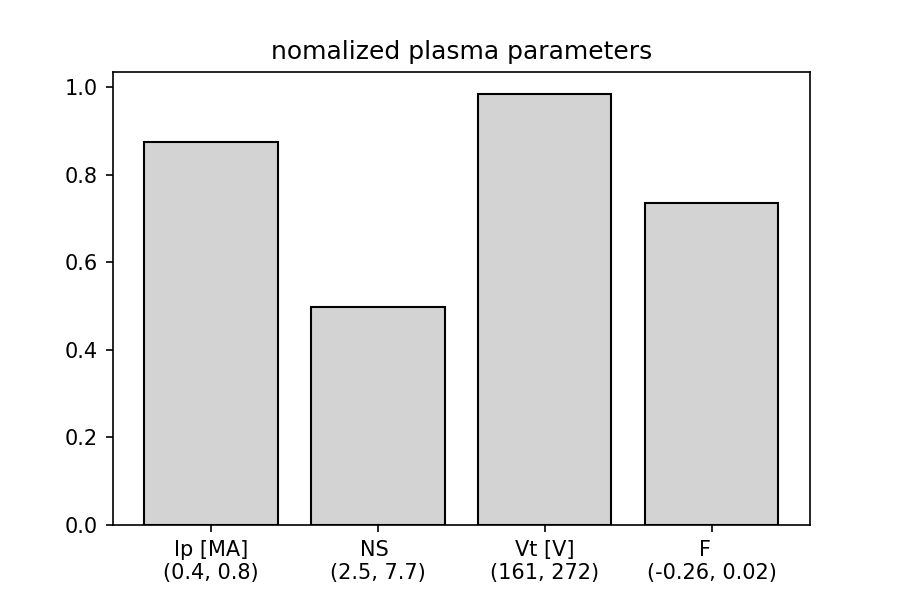
\includegraphics[height=4cm,trim={0.5cm 0cm 0.5cm 0cm  },clip]{img/STEP12_7c/Params_160.png}  }\\%
e.\subfigure{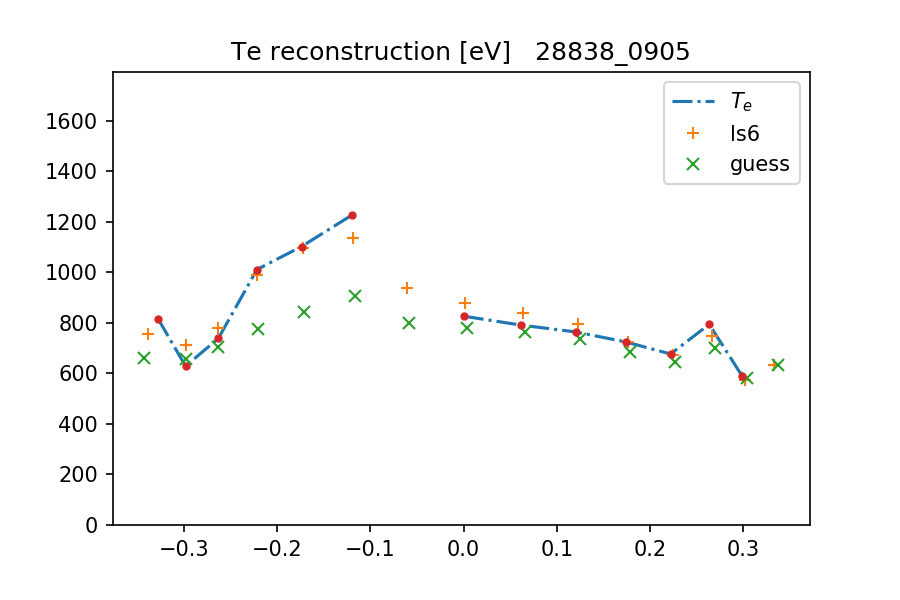
\includegraphics[height=4cm,trim={0.5cm 0cm 0.5cm 0.5cm},clip]{img/STEP12_7c/Te_rec_165.png}  }%   
\subfigure{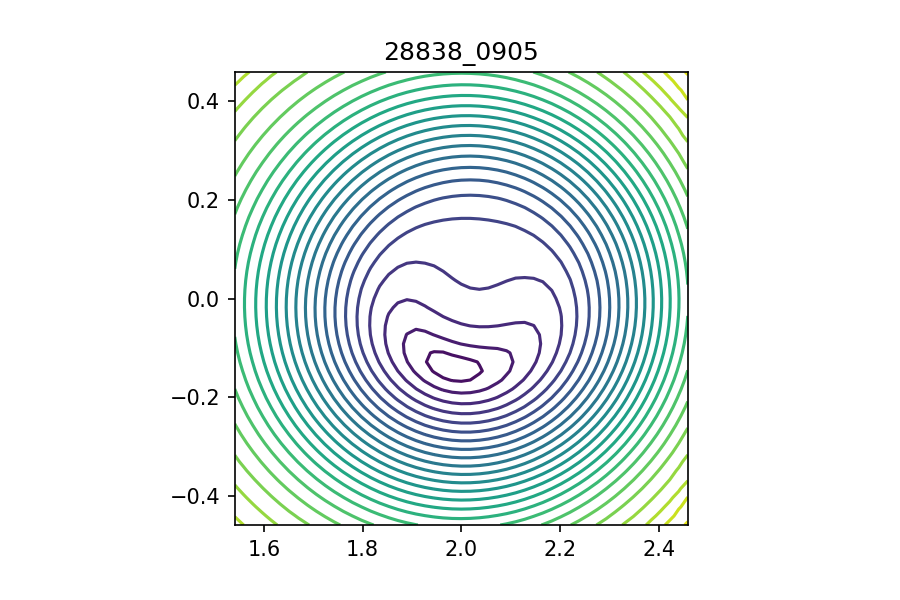
\includegraphics[height=4cm,trim={3cm   0   3.5cm 0    },clip]{img/STEP12_7c/Contour_165.png} }%  
\subfigure{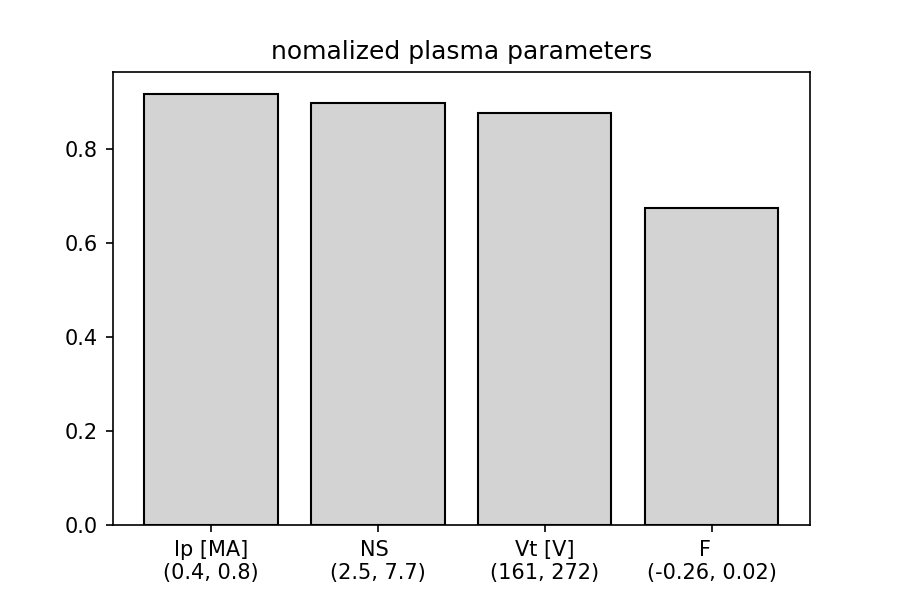
\includegraphics[height=4cm,trim={0.5cm 0cm 0.5cm 0cm  },clip]{img/STEP12_7c/Params_165.png}  }% 

% OLD
% \subfigure{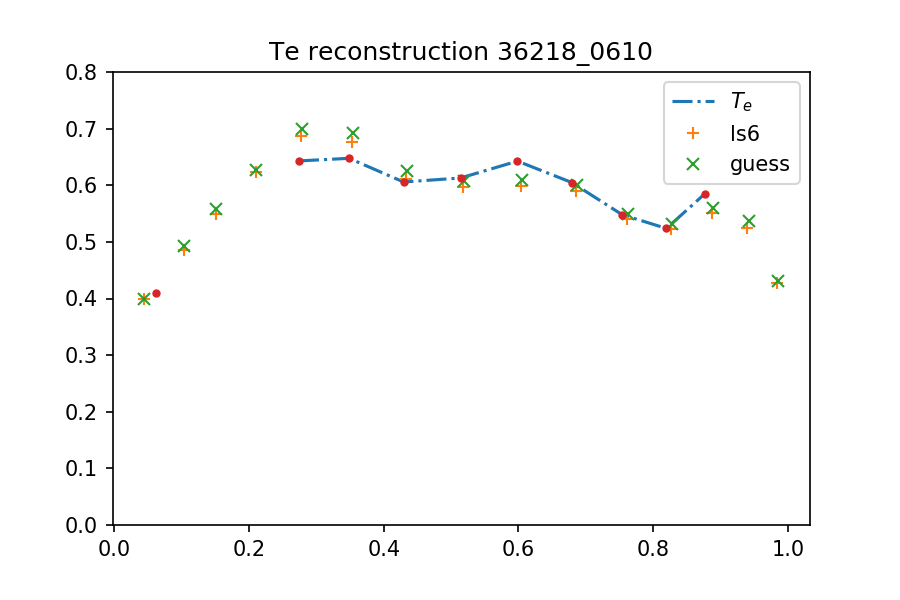
\includegraphics[height=4cm]{img/STEP12_7b/Te_rec_201.png}     }%
% \subfigure{\includegraphics[height=4cm]{img/STEP12_7b/Contour_201.png}    }%
% \subfigure{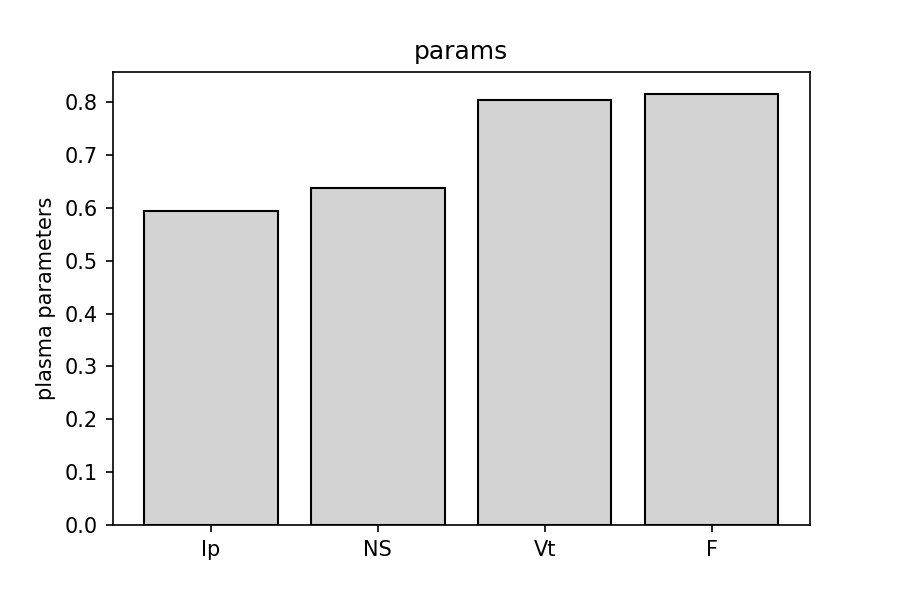
\includegraphics[height=4cm]{img/STEP12_7b/Params_201.png}     }\hfill
% \subfigure{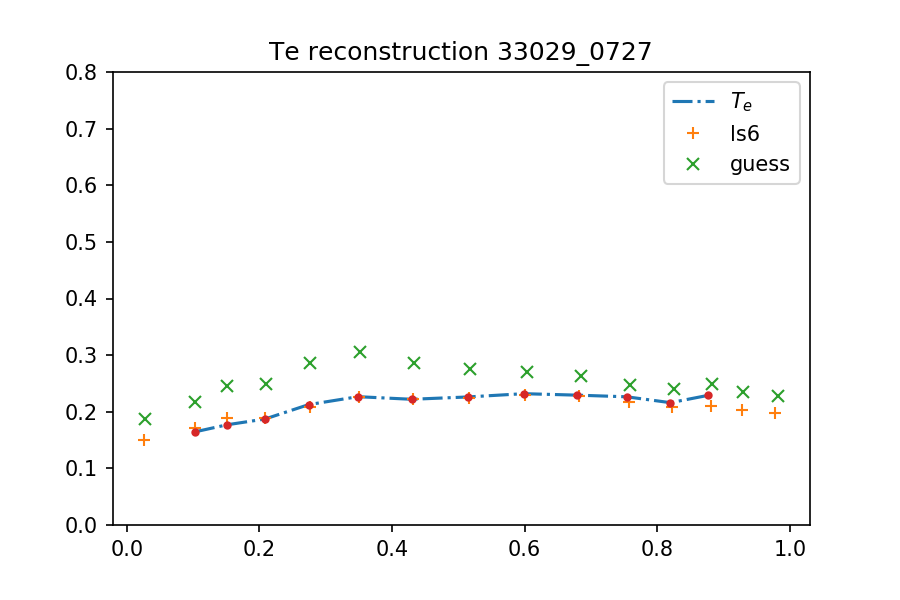
\includegraphics[height=4cm]{img/STEP12_7b/Te_rec_207.png}     }%
% \subfigure{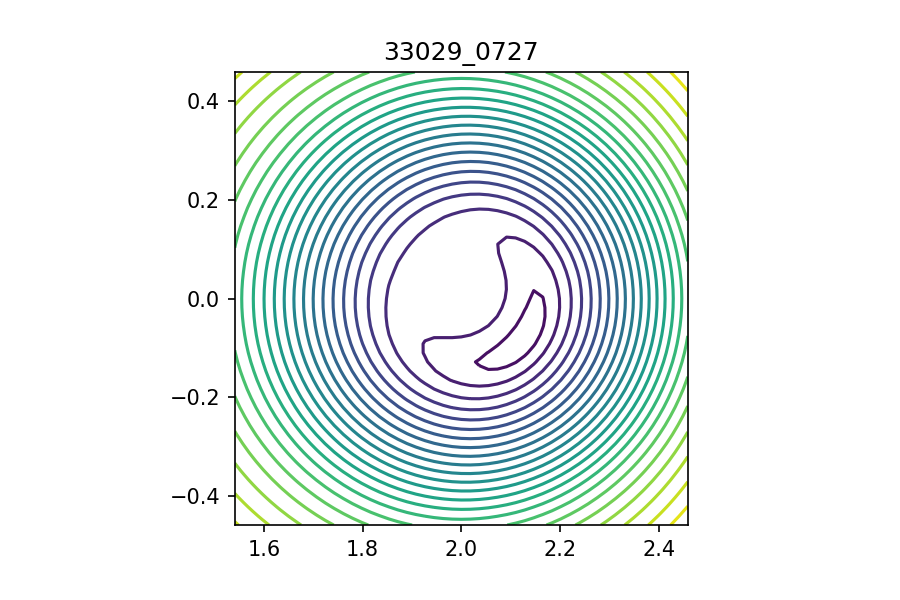
\includegraphics[height=4cm]{img/STEP12_7b/Contour_207.png}    }%
% \subfigure{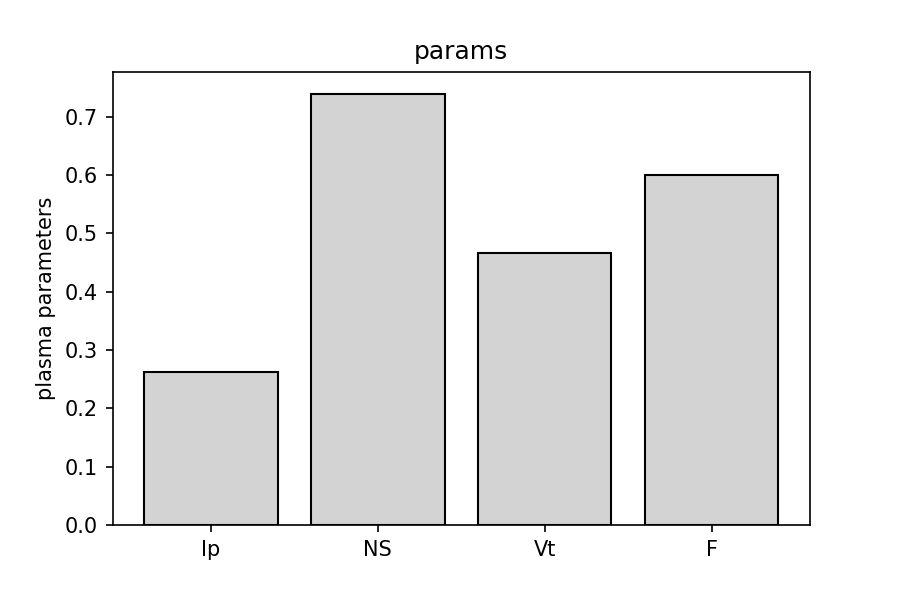
\includegraphics[height=4cm]{img/STEP12_7b/Params_207.png}     }\hfill
% \subfigure{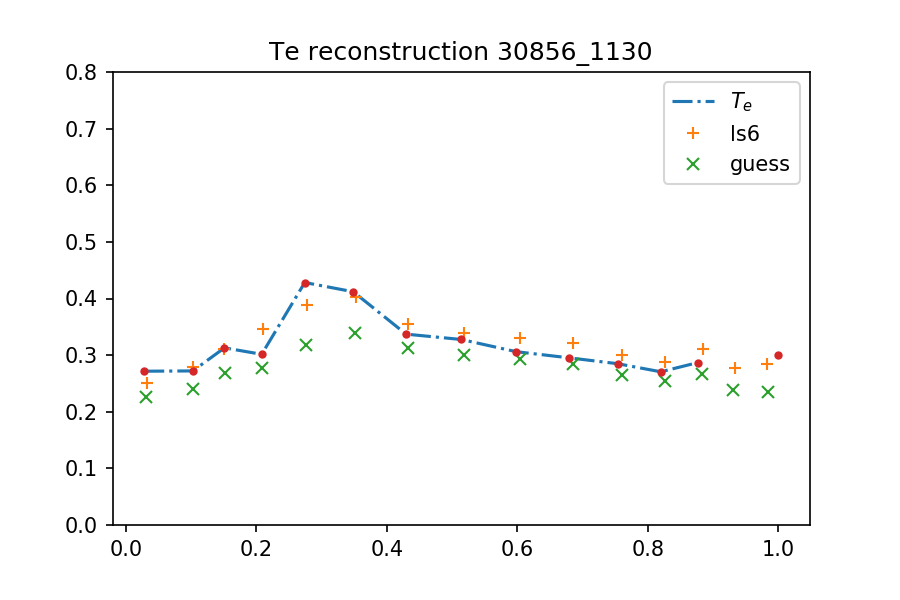
\includegraphics[height=4cm]{img/STEP12_7b/Te_rec_219.png}     }%
% \subfigure{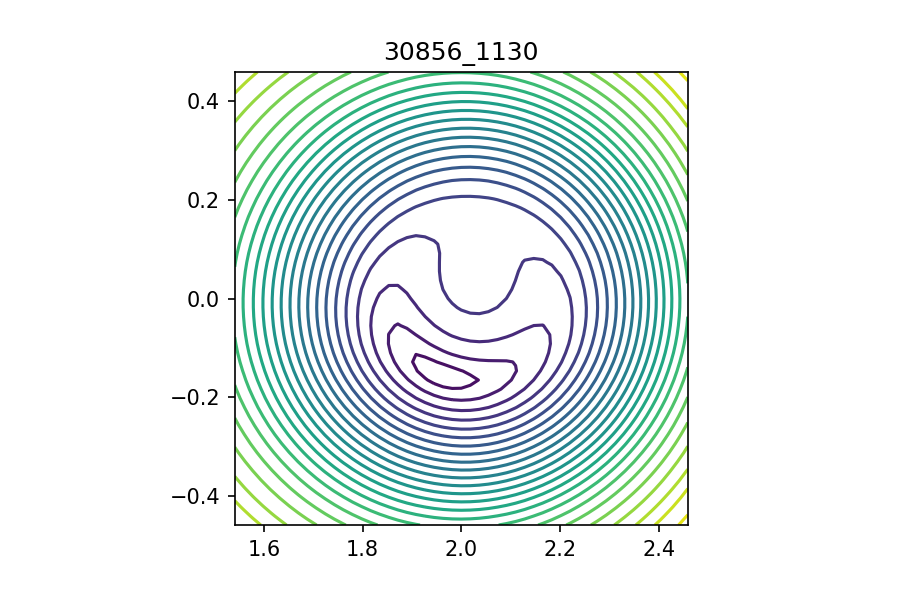
\includegraphics[height=4cm]{img/STEP12_7b/Contour_219.png}    }%
% \subfigure{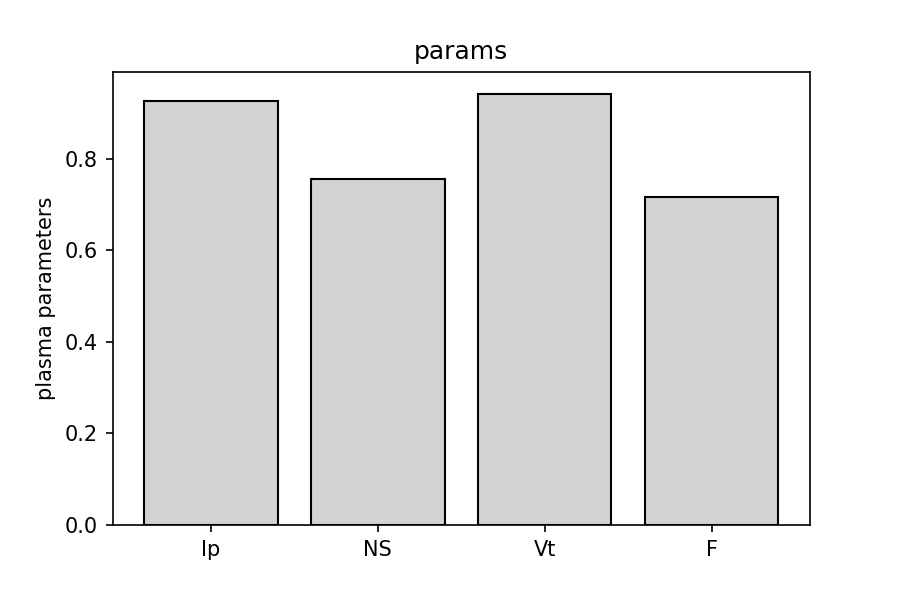
\includegraphics[height=4cm]{img/STEP12_7b/Params_219.png}     }\hfill
% \subfigure{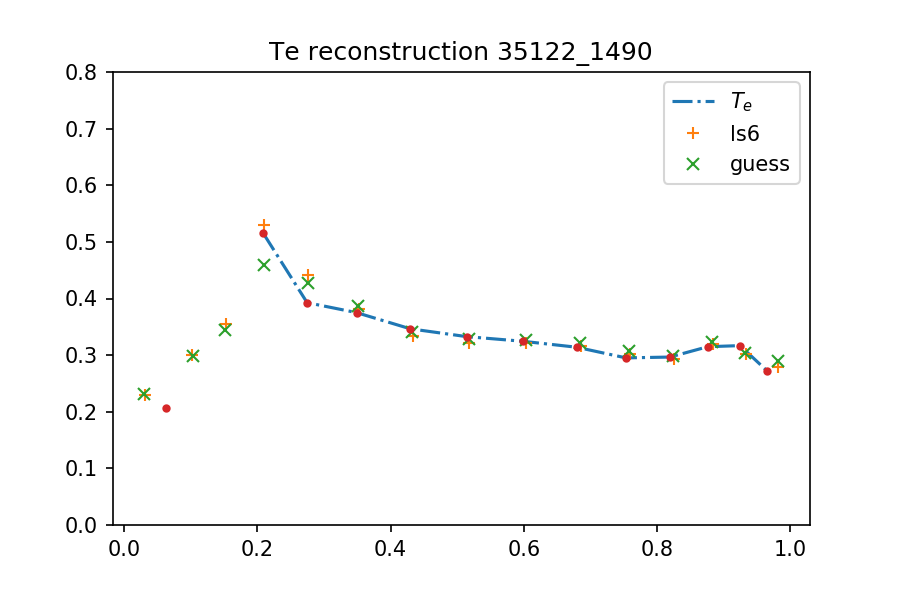
\includegraphics[height=4cm]{img/STEP12_7b/Te_rec_194.png}     }%
% \subfigure{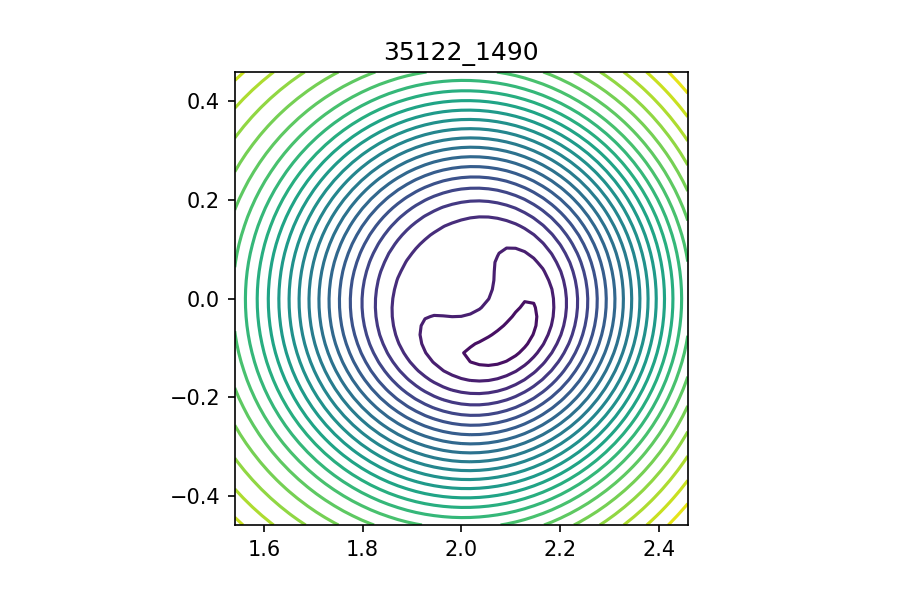
\includegraphics[height=4cm]{img/STEP12_7b/Contour_194.png}    }%
% \subfigure{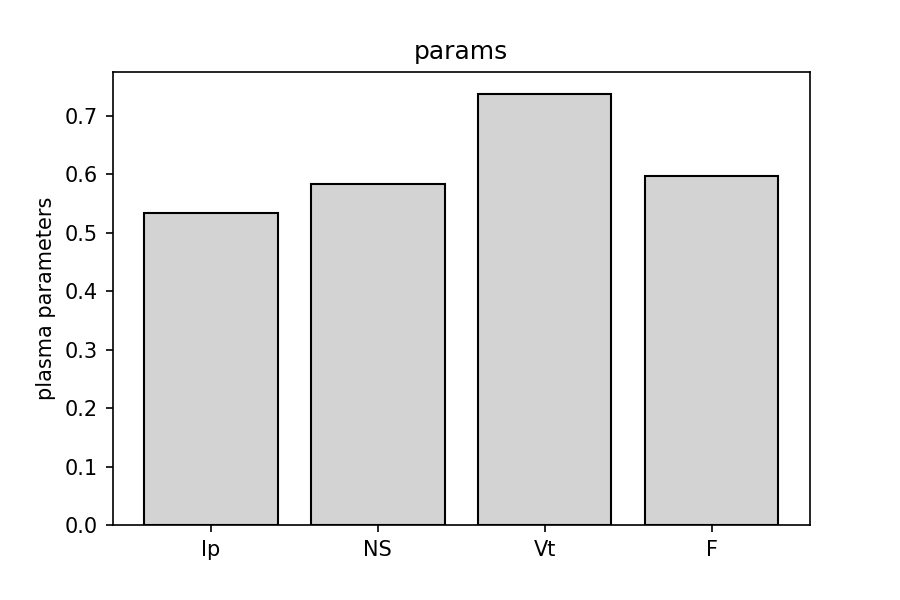
\includegraphics[height=4cm]{img/STEP12_7b/Params_194.png}     }\hfill

\caption{Reconstruction examples with plots of temperature profile, 2D reconstruction, and the related normalized plasma parameters. The temperature profile shows the real acquired $T_e$ from SXR3 with blue line (-.), the decoded profile from \VAE{6} in orange (+), and the inferred profile from magnetic configuration $(B_r, B_\varphi)$ at border. Three values of plasma current has been selected (a,b,c). A successful and failed phase identification is reported respectively in examples (d,e). }
\label{fig:Step_12_val}
\end{figure}
%
Among a set of tested signals we chose three that represent different possible values of plasma current \Figure{\ref{fig:Step_12_val}}(a,b,c), the remaining two examples are instead: a QSH shape with a phase that makes it clearly visible in the profile, and a case where instead the reconstruction failed to find the magnetic island at all \Figure{\ref{fig:Step_12_val}}(d,e).

The temperature reconstructions show in this case all the ML algorithms applied in one plot. The plot x-axis is the measure (in meters) of the impact parameter along the vertical axis orthogonal to the equatorial plane and passing through the center of the poloidal section. Thus it must be compared with the y-axis of the contour plot to appreciate the profile matching with the reconstructed flux surfaces. All measures have been fed through the networks normalized over the dataset, however in the plots the results have been scaled back to the original values in [eV].
The first curve represents the real measure SXR3 temperature profile with related acquired (and missing) data points.
The red markers are the available measures while the curve interrupts where any point is missing.
The orange (+) markers are the decoded profile that comes from the \bVAE{6} latent representation of measures. It shows the reconstruction of the profile missing data, and a smoothing/denoising effect associated with the \bVAE{6} itself.
The last over-imposed green (x) markers are the guessed profile. It is obtained decoding, again with \bVAE{6}, the latent configuration that has been in turn obtained by inference of the plasma parameters only.

It is worth noting that as the inference from the parameters is done with the respective latent configuration as label the guess is trying to reproduce the orange curve not the real measures. However a good match of these last two quantities is guaranteed by VAE.


To quantify the overall reconstruction a distribution of the mean absolute error has been obtained from the 3000 random samples of the validation dataset. The resulting histogram is shown in \Figure{\ref{fig:mae_histogram}} where a gaussian fit provides a standard deviation of 63 [eV], although the actual distribution seems not properly gaussian and leptokurtic (with a kurtosis of k=5.26). This means that the standard deviation is likely to be over-estimated but at the same time some relevant miss-reconstruction cases are present.
%
\begin{figure}
    \centering
    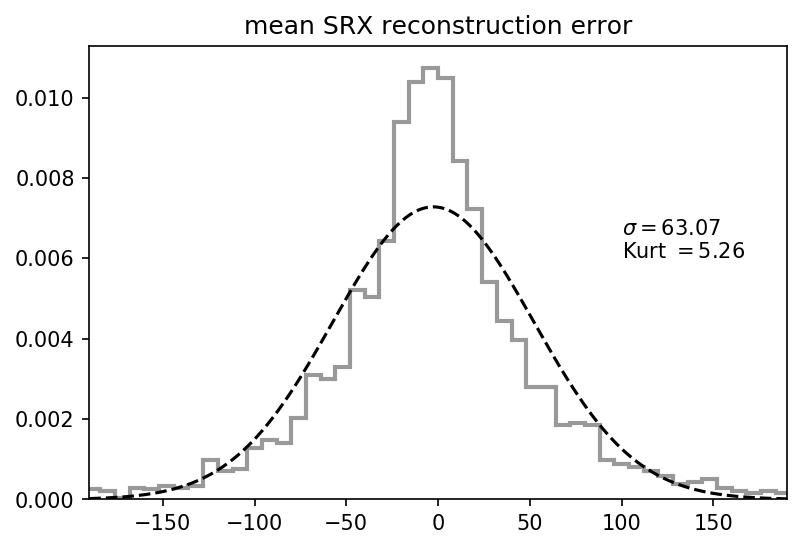
\includegraphics[height=6cm]{img/STEP12_7c/Mean_Absolute_Error.png}
    \caption{Mean absolute reconstruction error for SXR profile inference from magnetic parameters. The distribution is obtained from the validation dataset and shows a standard deviation of 63 [eV]. }
    \label{fig:mae_histogram}
\end{figure}
%
Those critical cases will be carefully selected and observed in a possible future continuation of this study to understand if a they are related to a limit of the network inference, or a physical explanation exists.





